\documentclass[a4paper, 12pt]{article}

\usepackage[top=2cm, bottom=2cm, left=2.5cm, right=2.5cm]{geometry}
\usepackage[utf8]{inputenc}
\usepackage{array}
\usepackage{verbatim}
\usepackage{graphicx}
\usepackage{hyperref}

\graphicspath{{img/}}

\begin{document}
\includegraphics{logo}\\
\textbf{UNIVERSIDADE ESTADUAL DE PONTA GROSSA} \\
SISTEMA UNIVERSIDADE ABERTA DO BRASIL - UAB \\
\underline{Licenciatura em Matemática | Polo UAB em Jacarezinho} \\
\textbf{ALUNO:} Ricardo Medeiros da Costa Junior   \textbf{RA:} 151774301 \\
\textbf{DISCIPLINA:} Instrumentação para o Ensino da Matemática IV \\
\textbf{ATIVIDADE:} Tarefa atividade 3 \\

\begin{enumerate}
\item Considere a questão abaixo e complete o que se pede: (Valor 2)
\begin{figure}[h!]
  \centering
  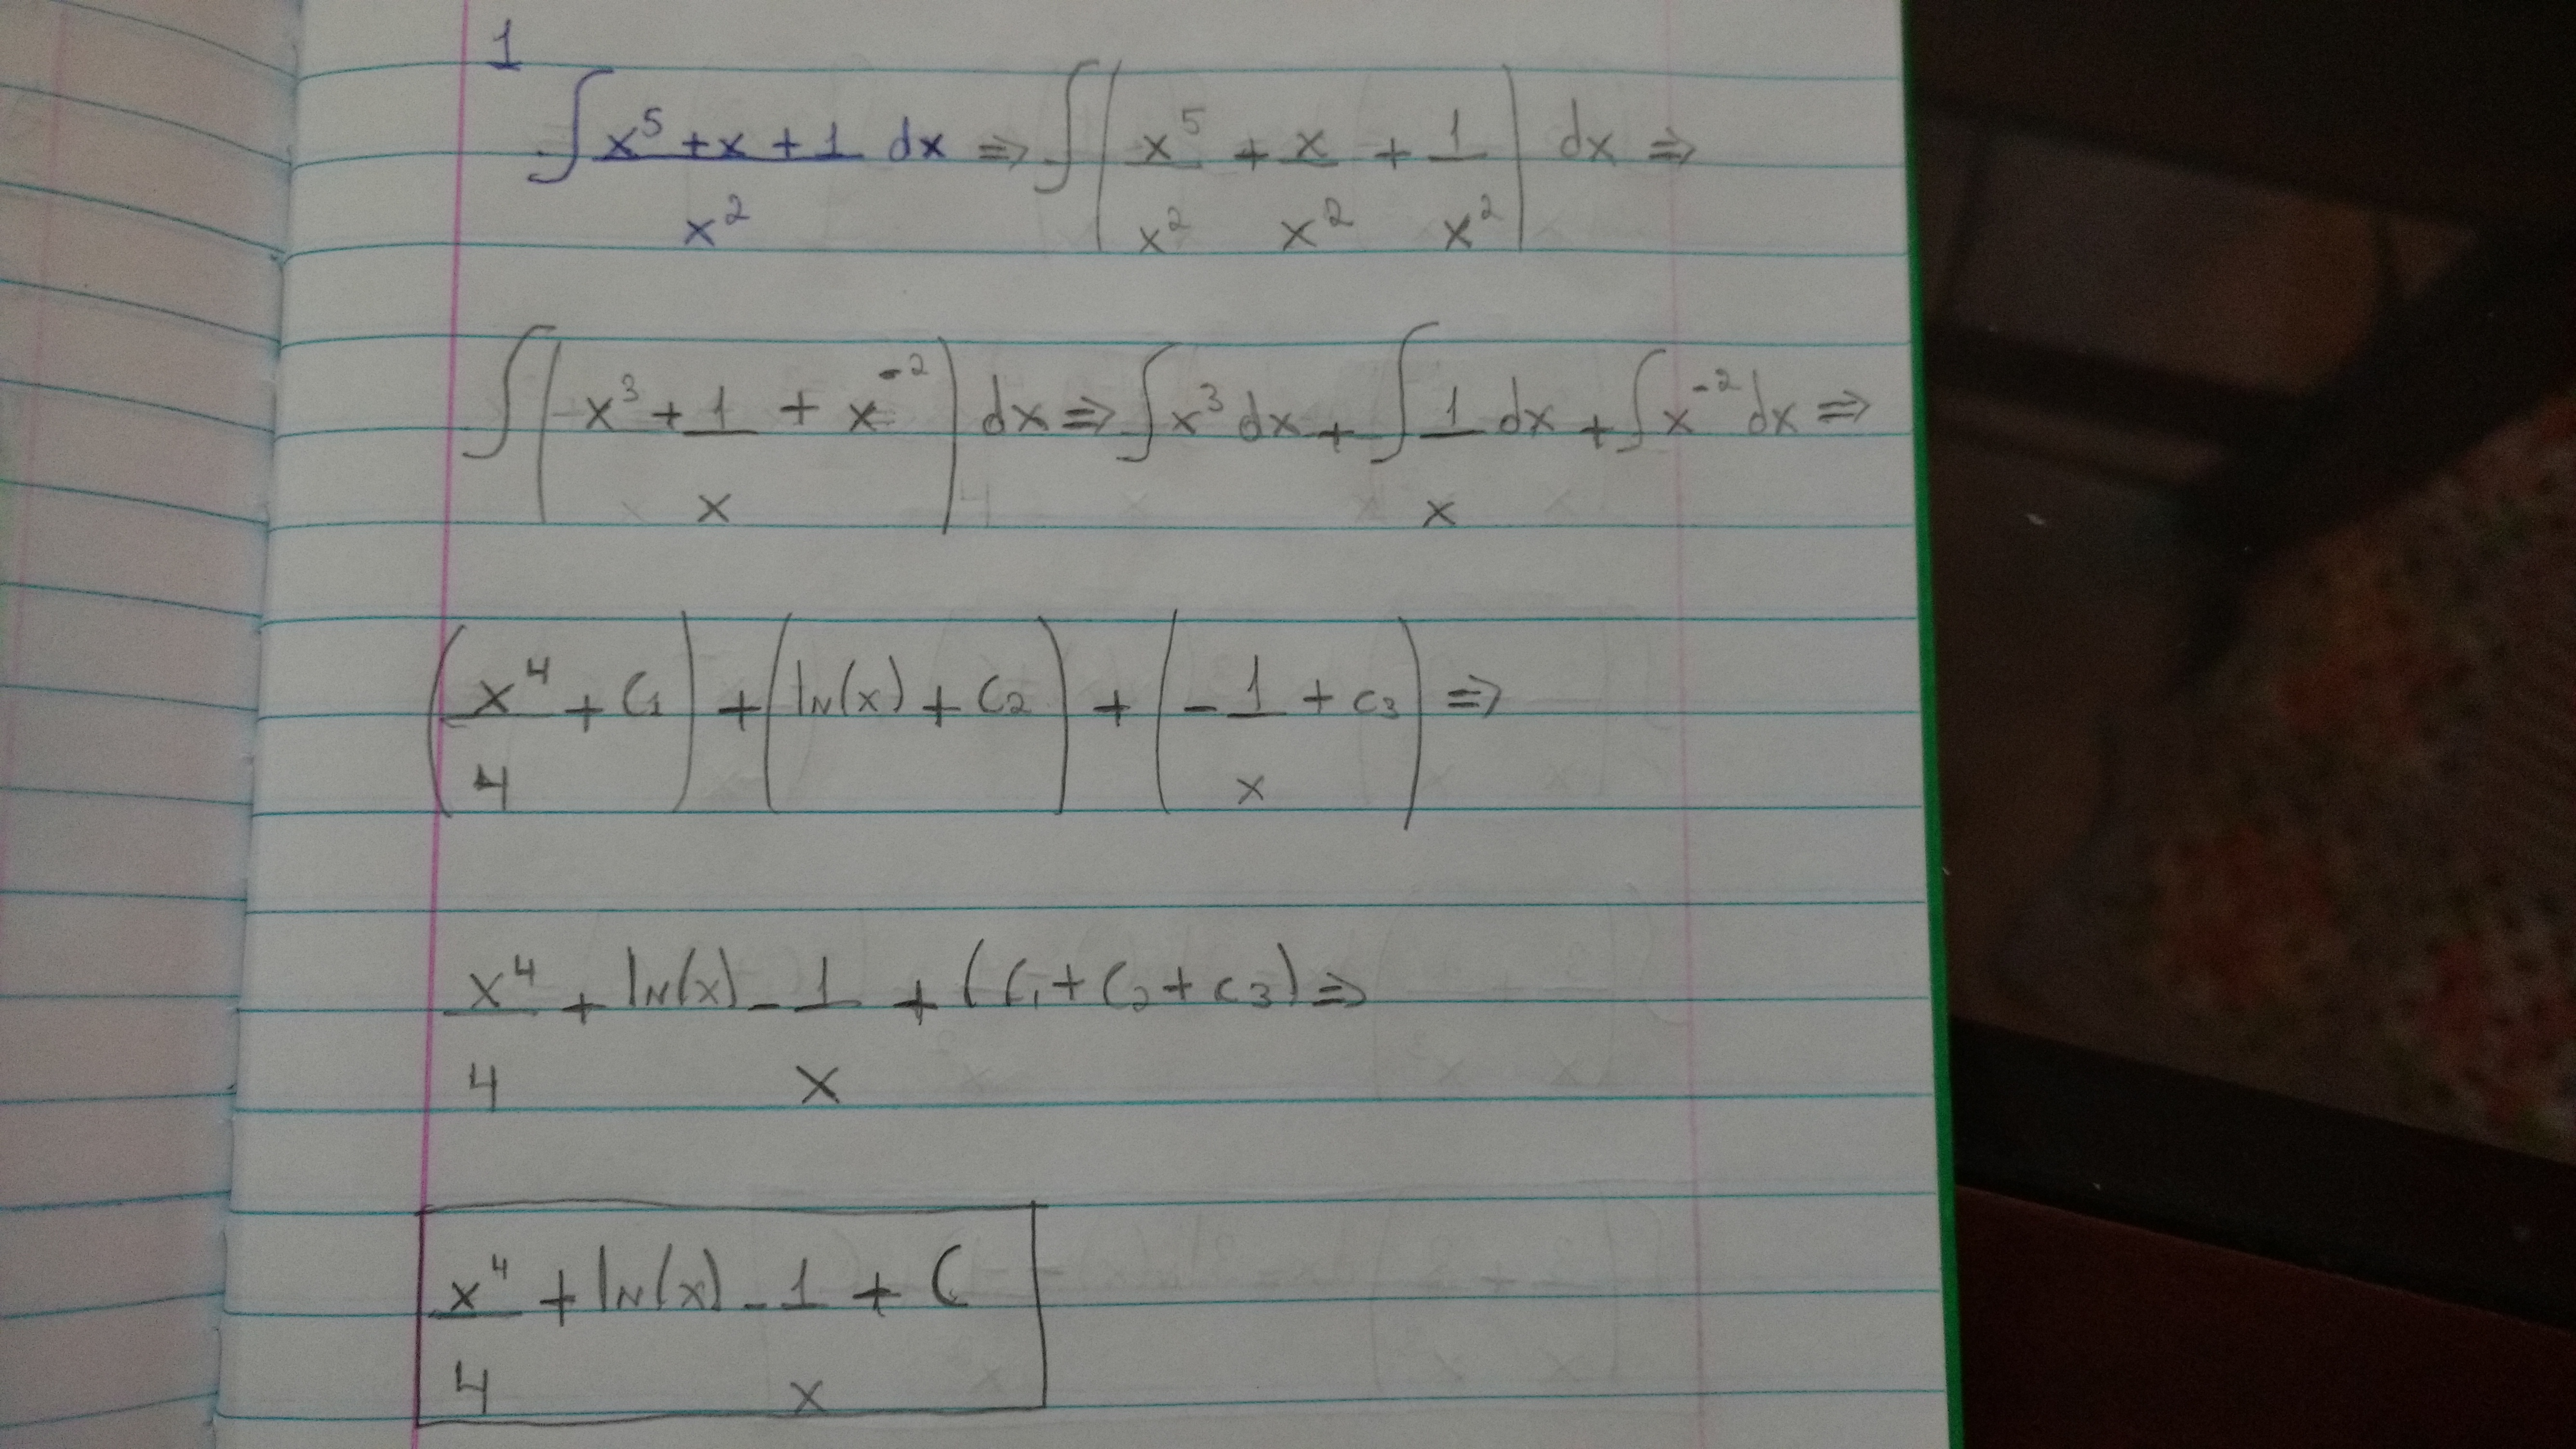
\includegraphics[width=0.7\textwidth]{1}
\end{figure} 
  \begin{enumerate}
  \item Conteúdo estruturante \\
    Geometrias, Números e Álgebra.
  \item Conteúdo Básico de Matemática\\
    Geometria Plana, Números Inteiros, Regra de três simples.
  \item Expectativas de aprendizagem\\
    29. Resolva situações-problema envolvendo figuras planas. 44. Resolva situações-problema envolvendo operações com números inteiros. 56. Resolva situações-problema envolvendo regra de três simples
  \end{enumerate}
\item Considere a questão abaixo e complete o que se pede: (Valor 2)
\begin{figure}[h!]
  \centering
  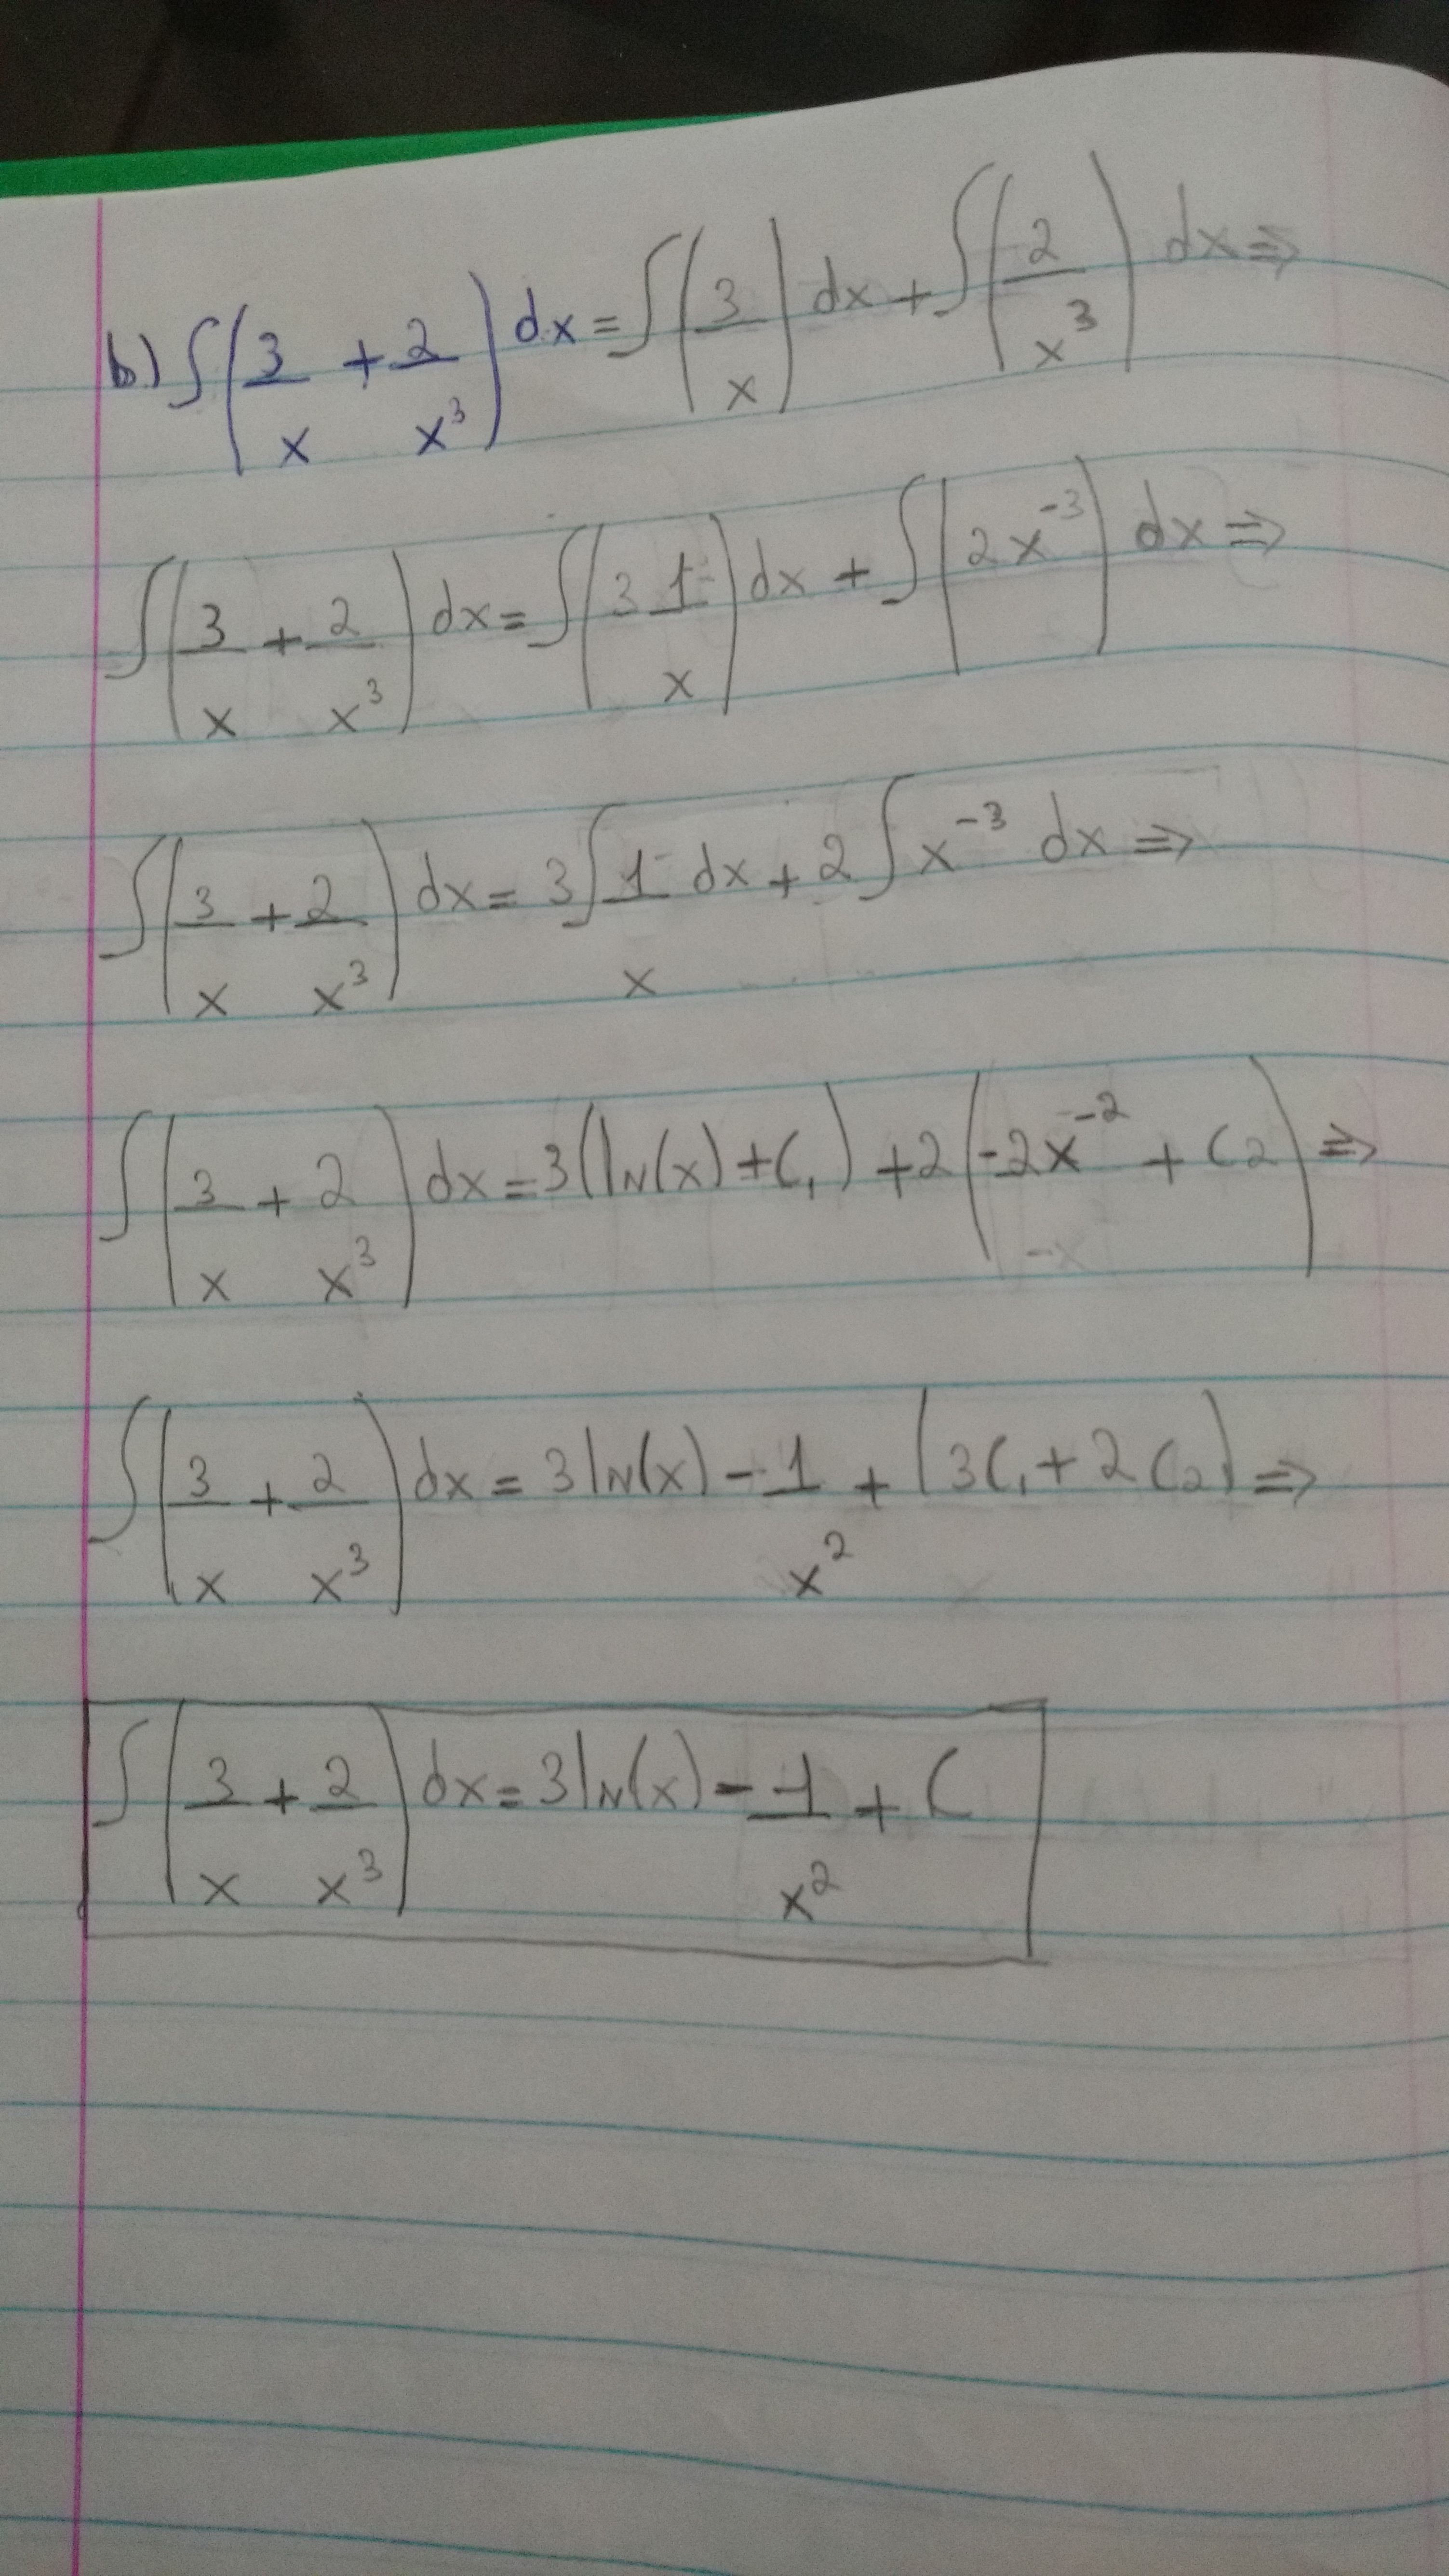
\includegraphics[width=0.7\textwidth]{2}
\end{figure} 
  \begin{enumerate}
  \item Conteúdo estruturante\\
    Funções.    
  \item Conteúdo Básico de Matemática\\
    Progressão Aritmética.
  \item Expectativas de aprendizagem\\
    213. Resolva situações-problema envolvendo Progressões Aritméticas e/ou Geométricas.
  \end{enumerate}
\item Considere a questão abaixo e complete o que se pede: (Valor 2)
\begin{figure}[h!]
  \centering
  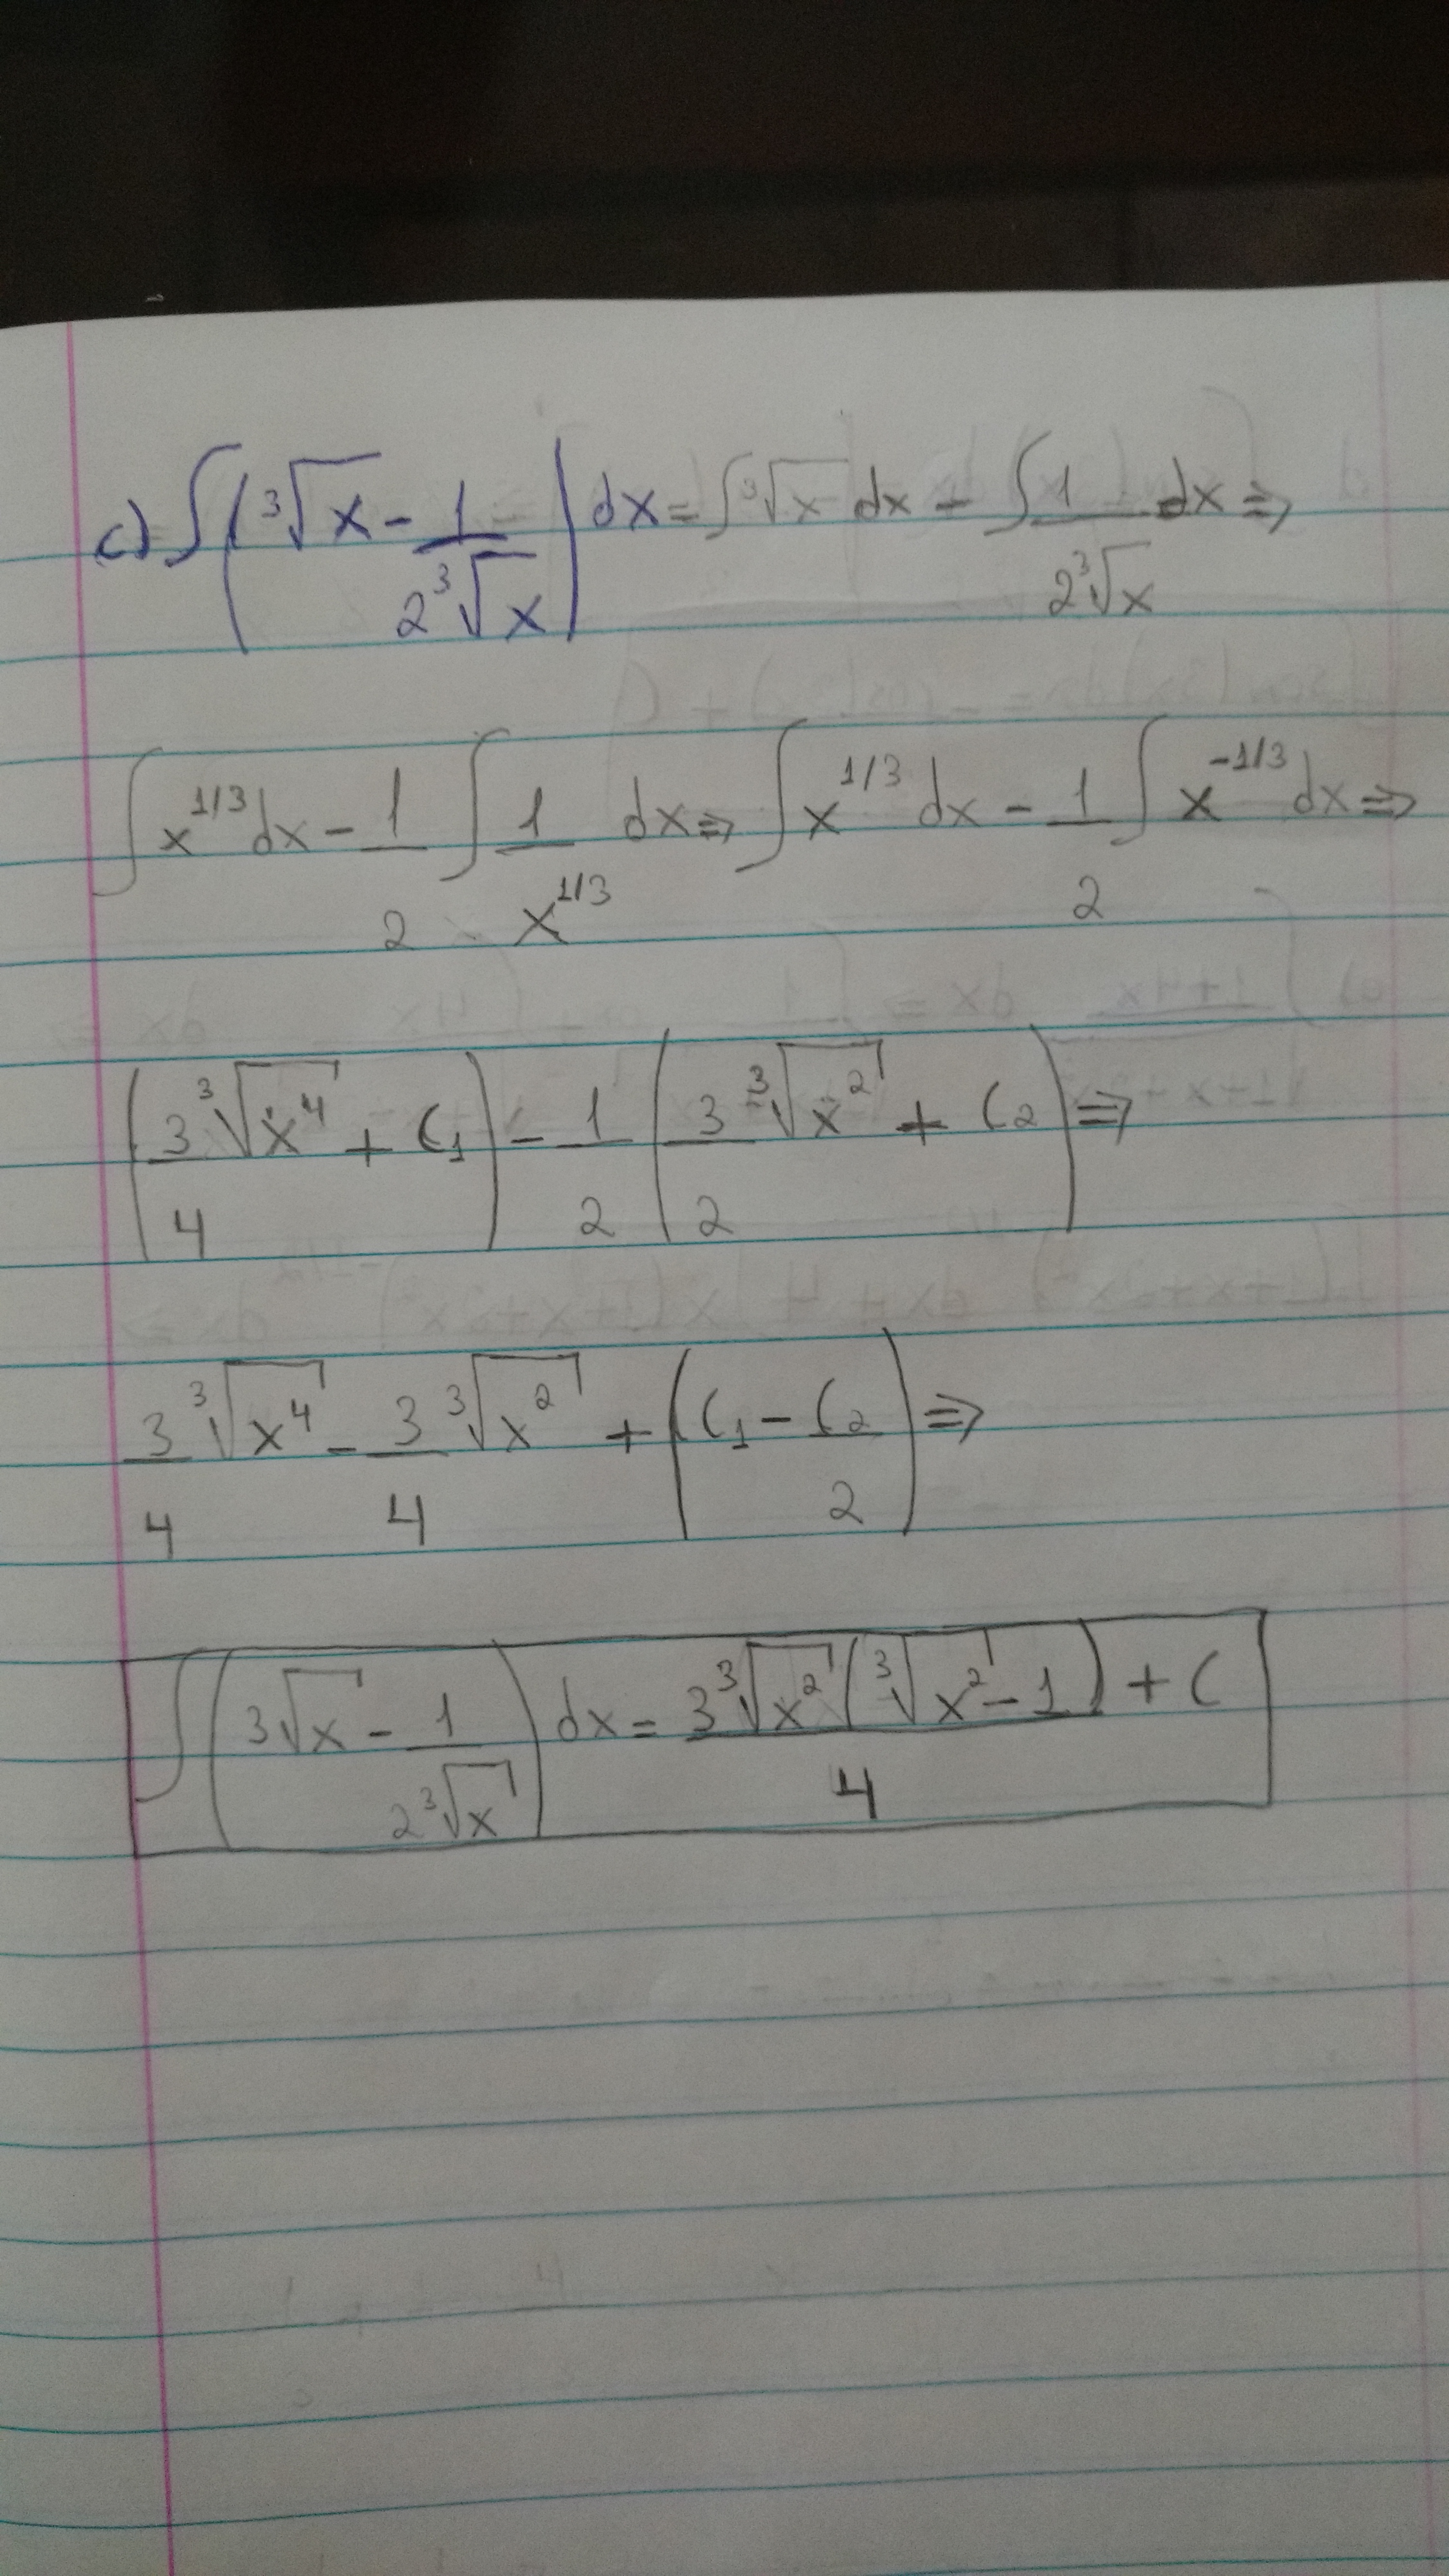
\includegraphics[width=0.7\textwidth]{3}
\end{figure} 
  \begin{enumerate}
  \item Conteúdo estruturante\\
    Tratamento de Informação.
  \item Conteúdo Básico de Matemática\\
    Estudo das probabilidades
  \item Expectativas de aprendizagem\\
    248. Resolva situações-problemas envolvendo o cálculo de probabilidades.
  \end{enumerate}
\item Considere a questão abaixo e complete o que se pede: (Valor 2)
\begin{figure}[h!]
  \centering
  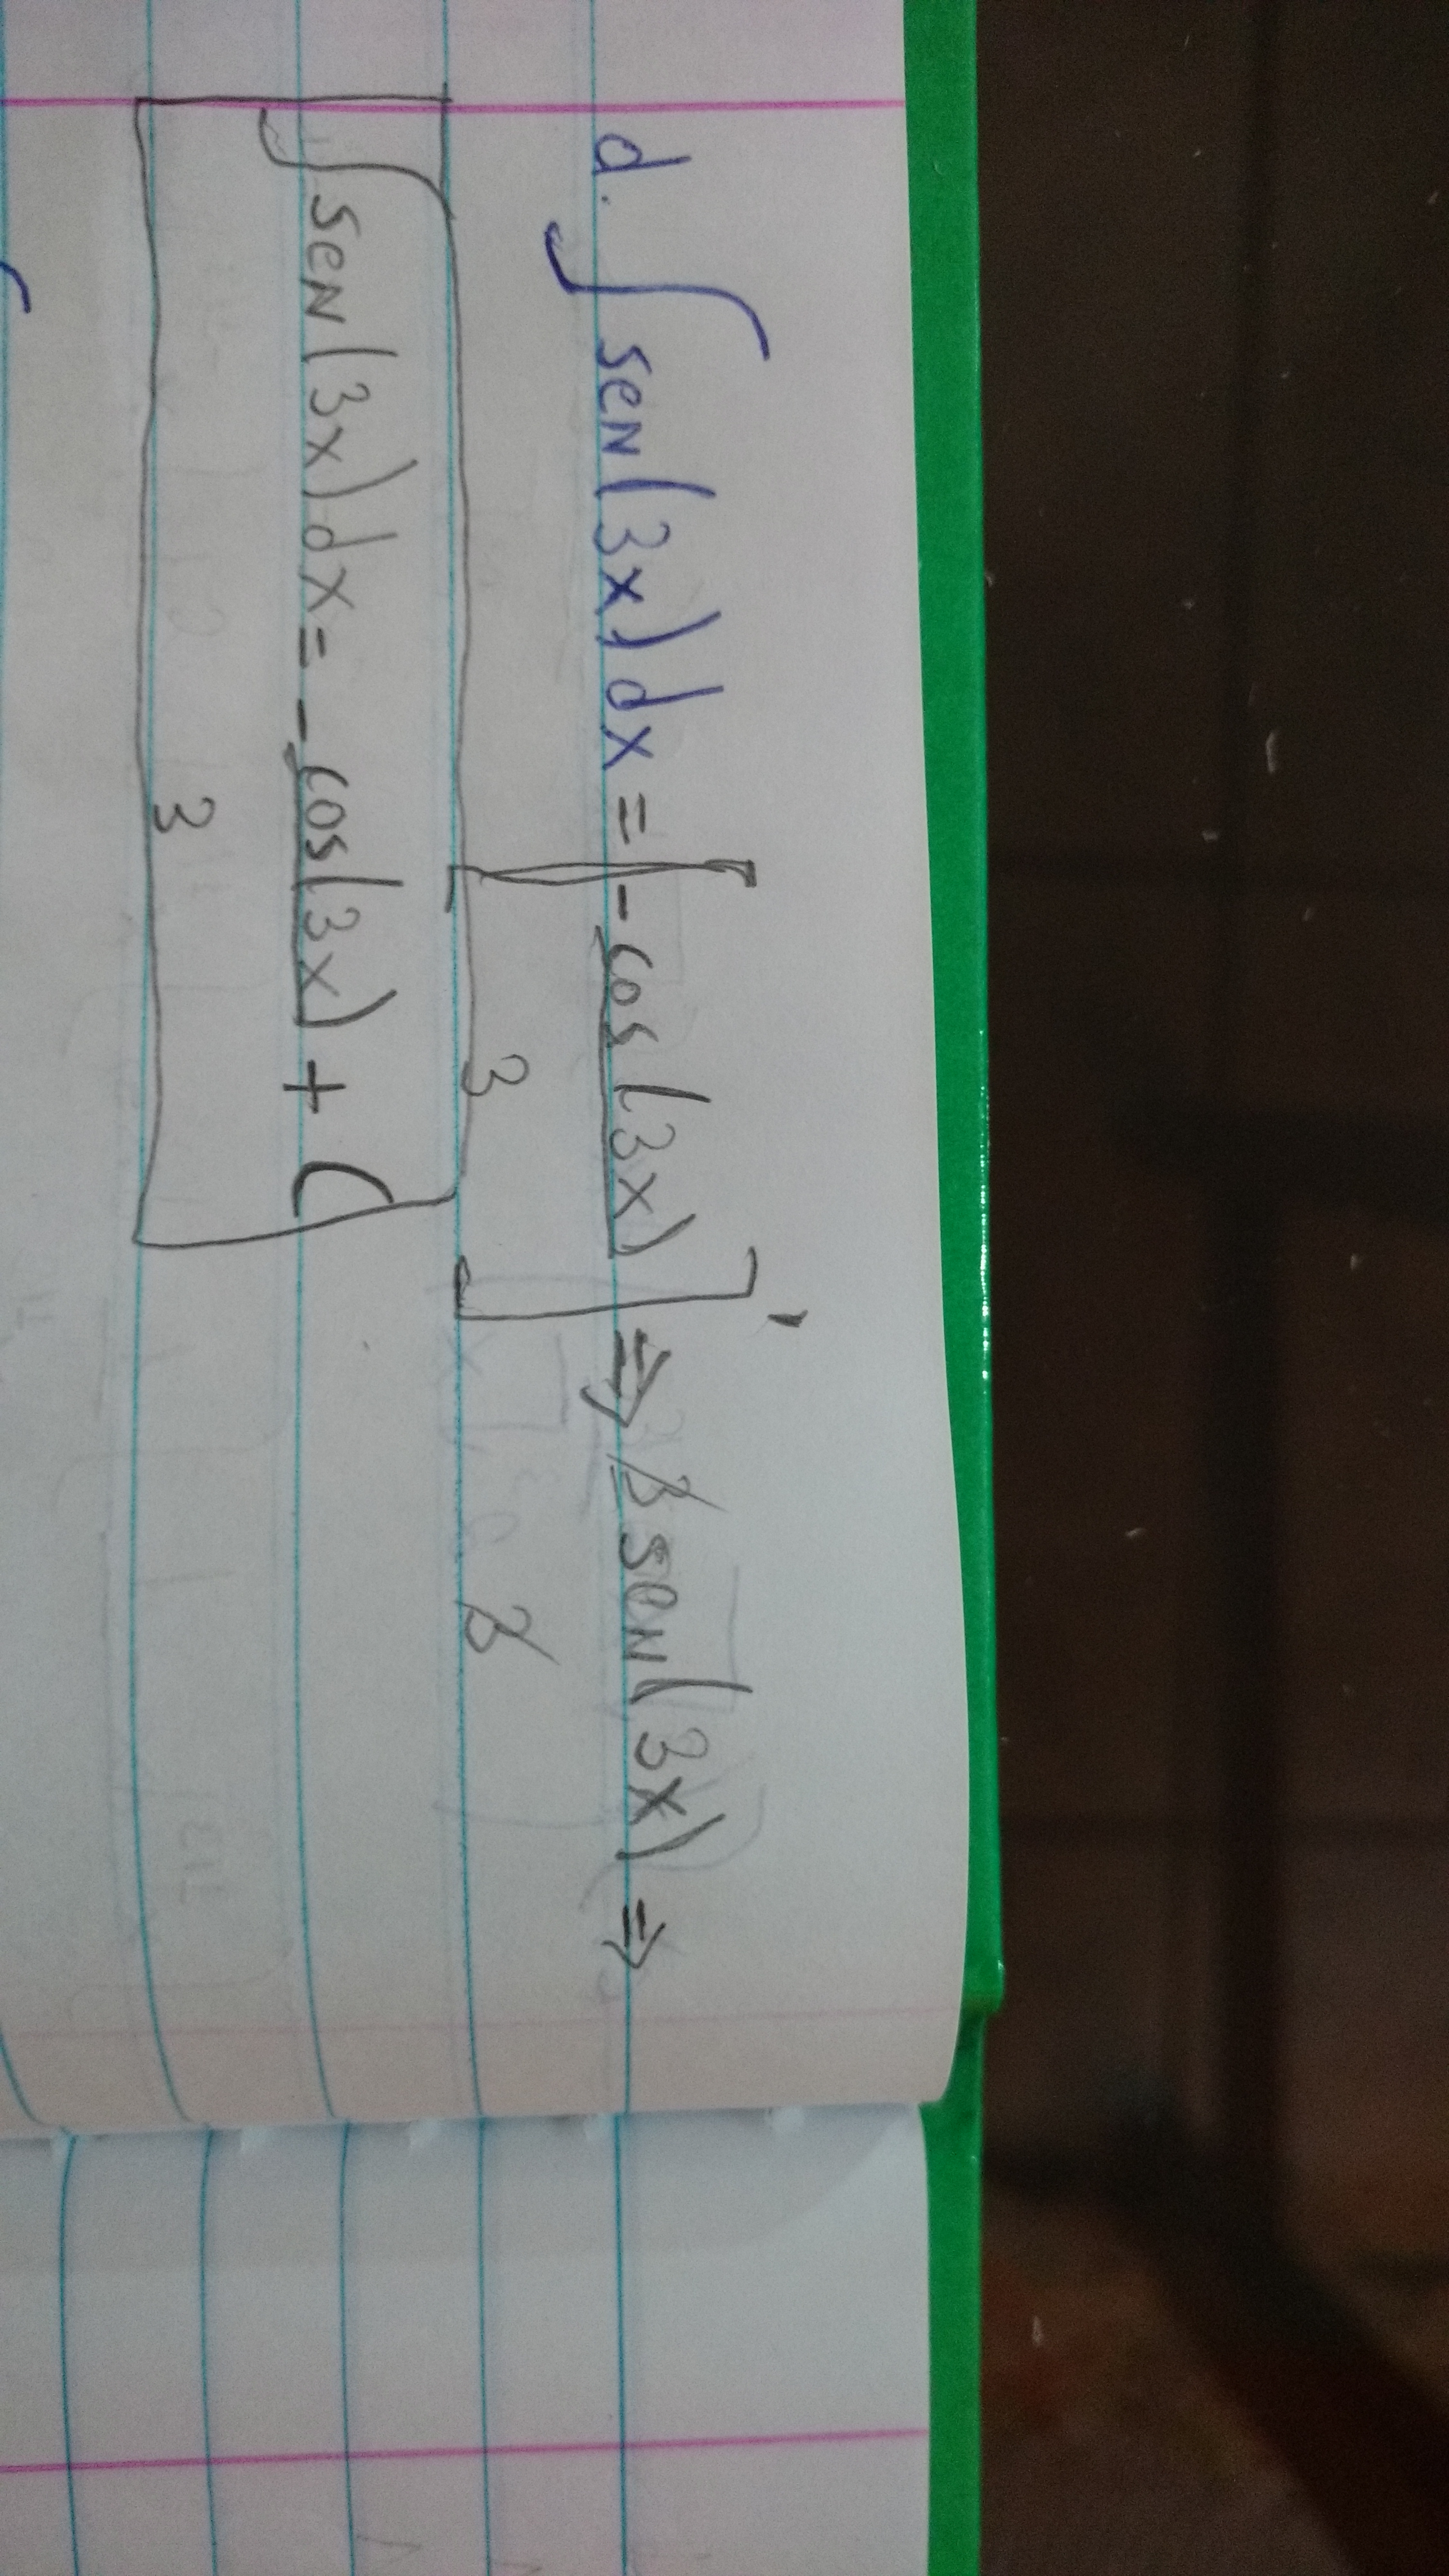
\includegraphics[width=0.7\textwidth]{4}
\end{figure} 
  \begin{enumerate}
  \item Conteúdo estruturante\\
    Geometrias.
  \item Conteúdo Básico de Matemática\\
    Geometria Plana.
  \item Expectativas de aprendizagem\\
    219. Resolva situações-problema envolvendo posições relativas entre pontos, retas e planos. 230. Resolva situações-problema envolvendo o cálculo de áreas de superfícies, volume e capacidade de sólidos geométricos
  \end{enumerate}
\item Considere a questão abaixo e complete o que se pede: (Valor 2)
\begin{figure}[h!]
  \centering
  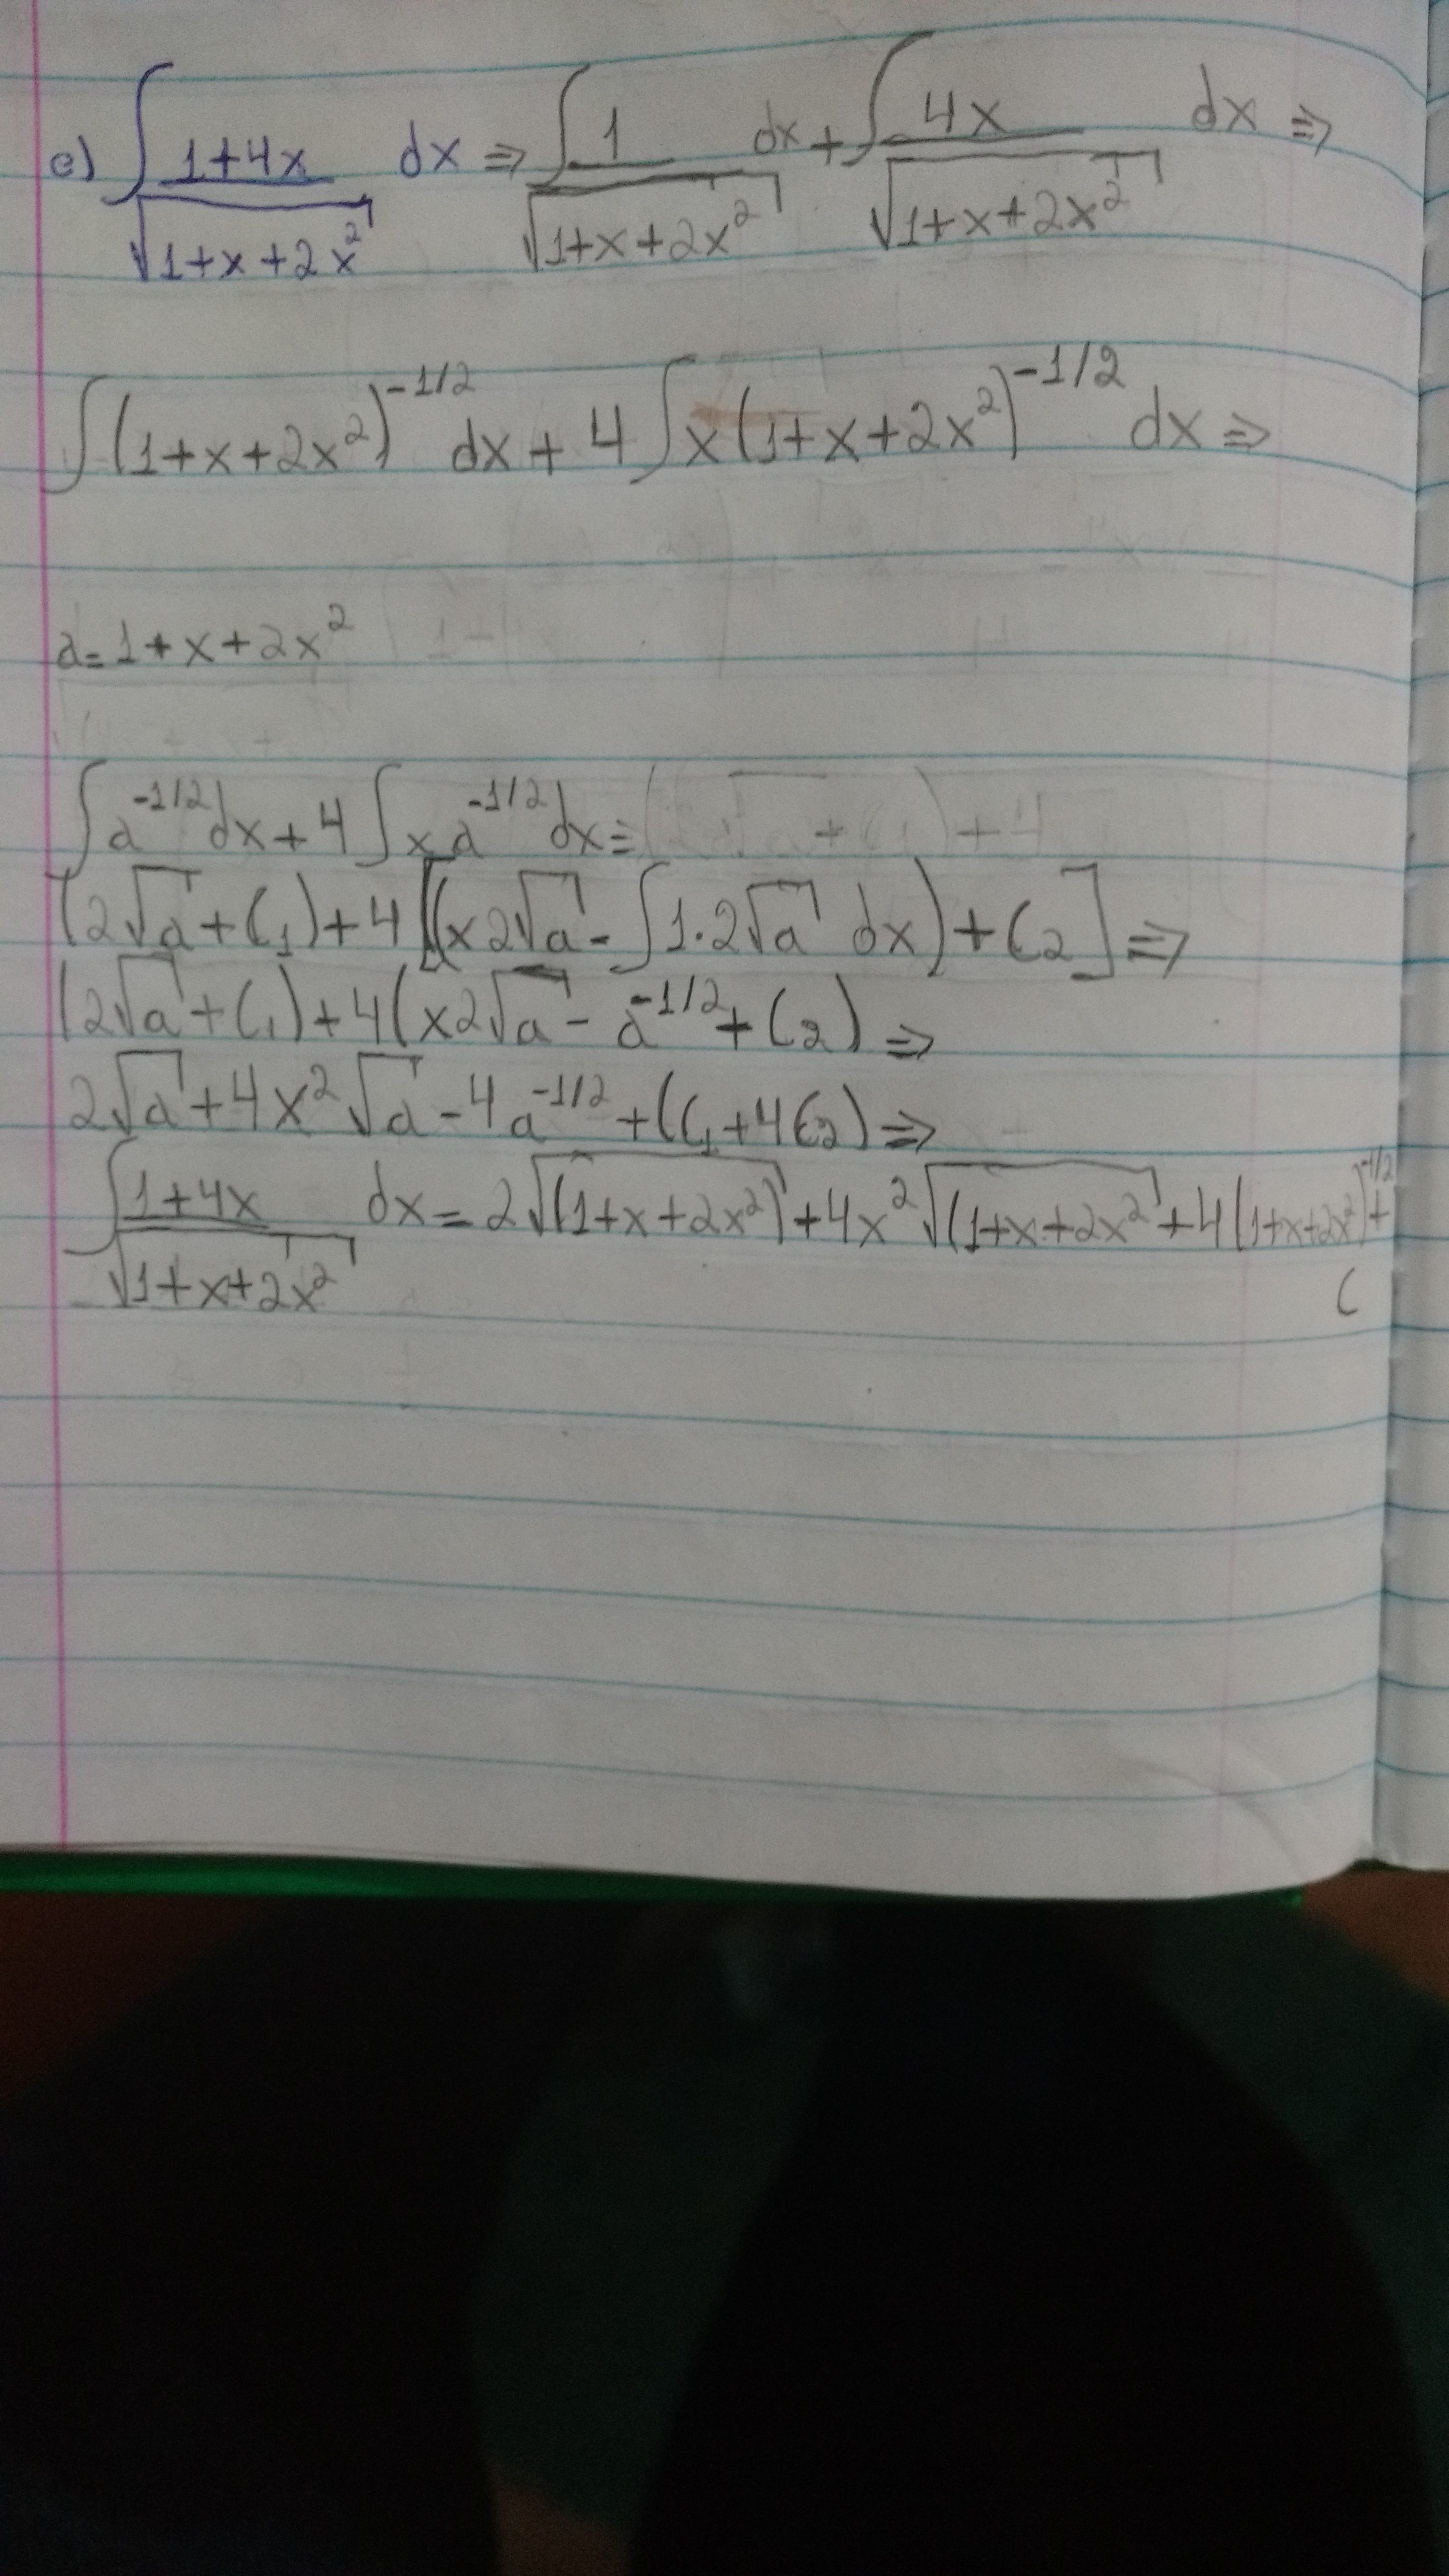
\includegraphics[width=0.5\textwidth]{5}
\end{figure} 
  \begin{enumerate}
  \item Conteúdo estruturante\\
    Números e Álgebra.
  \item Conteúdo Básico de Matemática\\
    Números Inteiros.
  \item Expectativas de aprendizagem\\
    44. Resolva situações-problema envolvendo operações com números inteiros.
  \end{enumerate}

\end{enumerate}
\end{document}
